% To je predloga za poročila o domačih nalogah pri predmetih, katerih
% nosilec je Blaž Zupan. Seveda lahko tudi dodaš kakšen nov, zanimiv
% in uporaben element, ki ga v tej predlogi (še) ni. Več o LaTeX-u izveš na
% spletu, na primer na http://tobi.oetiker.ch/lshort/lshort.pdf.
%
% To predlogo lahko spremeniš v PDF dokument s pomočjo programa
% pdflatex, ki je del standardne instalacije LaTeX programov.

\documentclass[a4paper,11pt]{article}
\usepackage{a4wide}
\usepackage{fullpage}
\usepackage[utf8x]{inputenc}
\usepackage[slovene]{babel}
\selectlanguage{slovene}
\usepackage[toc,page]{appendix}
\usepackage[pdftex]{graphicx} % za slike
\usepackage{setspace}
\usepackage{color}
\definecolor{light-gray}{gray}{0.95}
\usepackage{listings} % za vključevanje kode
\usepackage{hyperref}
\usepackage{titlesec}
\usepackage{float}


\renewcommand{\baselinestretch}{1.2} % za boljšo berljivost večji razmak
\renewcommand{\appendixpagename}{\normalfont\Large\bfseries{Priloge}}


\titleformat{name=\section}[runin]
  {\normalfont\bfseries}{}{0em}{}
\titleformat{name=\subsection}[runin]
  {\normalfont\bfseries}{}{0em}{}


% header
\makeatletter
\def\@maketitle{%
  \noindent
  \begin{minipage}{2in}
  \@author
  \end{minipage}
  \hfill
  \begin{minipage}{1.2in}
  \textbf{\@title}
  \end{minipage}
  \hfill
  \begin{minipage}{1.2in}
  \@date
  \end{minipage}
  \par
  \vskip 1.5em}
\makeatother


\lstset{ % nastavitve za izpis kode, sem lahko tudi kaj dodaš/spremeniš
language=Python,
basicstyle=\footnotesize,
basicstyle=\ttfamily\footnotesize\setstretch{1},
backgroundcolor=\color{light-gray},
}


% Naloga
\title{Naloga 5}
% Ime Priimek (vpisna)
\author{Jakob Udovič (63180301)}
\date{\today}

\begin{document}

\maketitle

\section{Regularizacija.}

Za regularizacije sem si izbral 3 različne vrednosti lambda: 0.01, 0.001 in 0.0001
Najboljšpi rezultat dobim z vrednostjo 0.001. Tu se najbolje vidijo meje med razredoma.


Namreč naše značilke imajo veliko več dimenzij (27), kot pa jih imamo mi na voljo za prikaz/vizualizacijo podatkov.
To pomeni, da bomo v večdimenzionalnem prostoru lažje določili mejo med razredoma s hiperravnino, v 2D prostoru pa si lahko pomagamo na drug način.

V tem primeru lahko pri 0.001 vrednosti lambde vidimo različne verjetnosti (odtenke barv) za primere na robu.
Tako na nek način ohranjamo "moč" meje logistične regresije pri prikazu le-te v prostoru s precej manj dimenzijami.

Rezultat je tako smiseln, saj pri lambda=0 ne vidimo nobenega prehoda med razredoma.

\begin{figure}[H]
\begin{center}
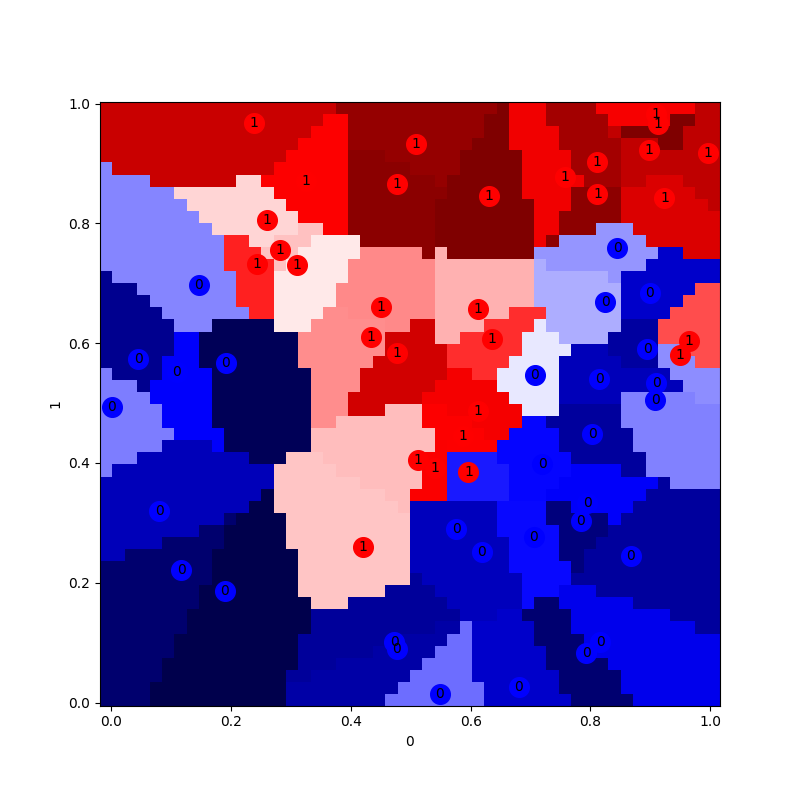
\includegraphics[scale=0.3]{01.png}
\caption{Napoved pri lambda = 0.01}
\label{slika1}
\end{center}
\end{figure}

\begin{figure}[H]
\begin{center}
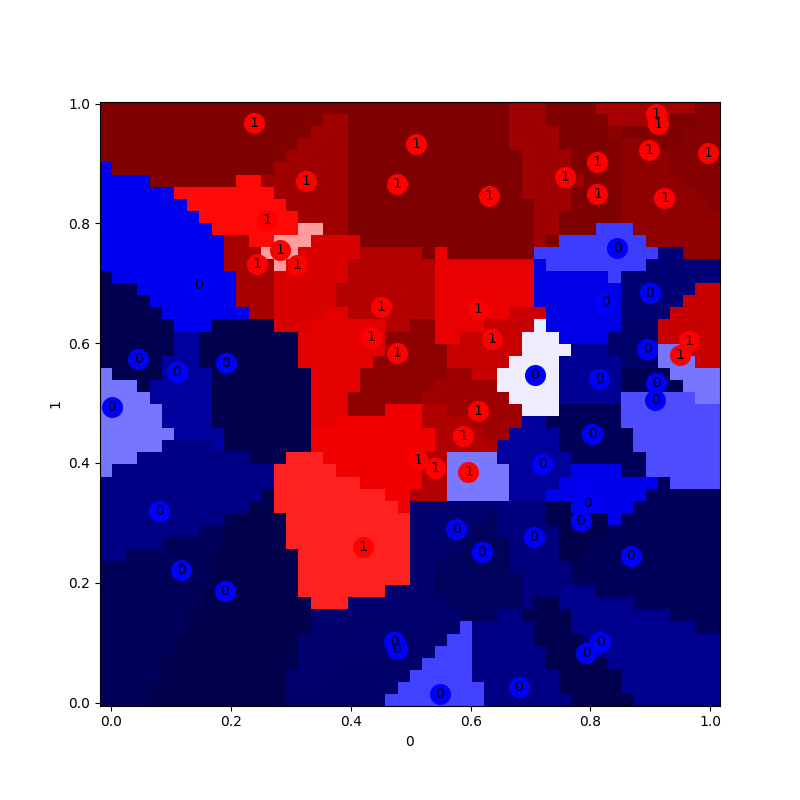
\includegraphics[scale=0.3]{001.png}
\caption{Napoved pri lambda = 0.001}
\label{slika2}
\end{center}
\end{figure}

\begin{figure}[H]
\begin{center}
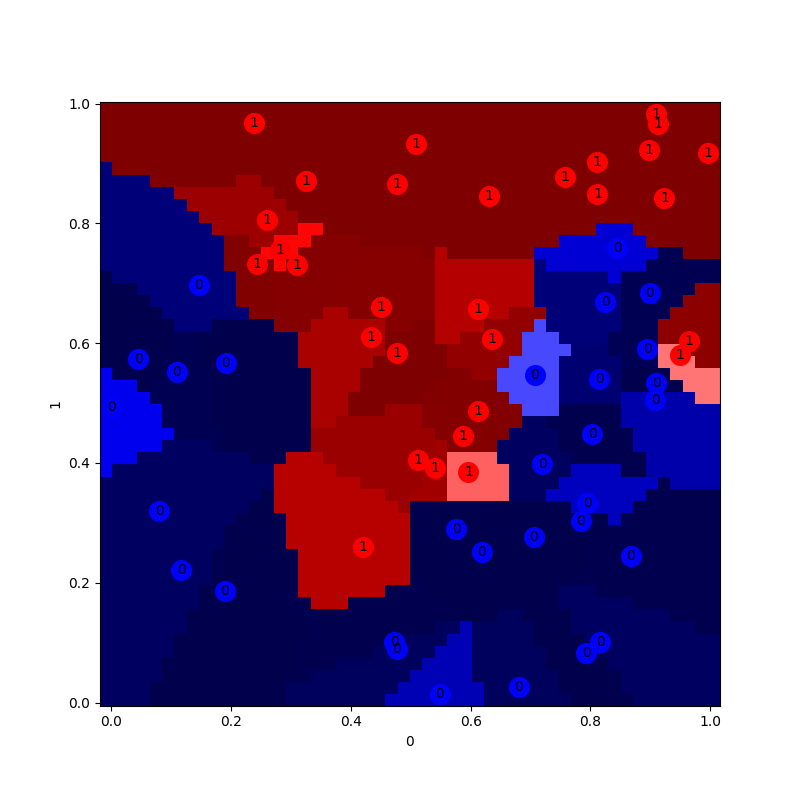
\includegraphics[scale=0.3]{0001.png}
\caption{Napoved pri lambda = 0.0001}
\label{slika3}
\end{center}
\end{figure}

\section{Točnosti.}
\begin{table}[htbp]
\caption{Ocene točnosti CA in CV predikcij pri različnih vrednostih lambda.}
\label{tab1}
\begin{center}
\begin{tabular}{llp{3cm}}
\hline
lambda & točnost CA & točnost CV (cross validation/prečno preverjanje) \\
\hline
0.00001 & 1 & 0.667\\
0.0001 & 1 & 0.683\\
0.001 & 0.967 &  0.7\\
0.01 & 0.95 & 0.683\\
0.1 & 0.917 & 0.683\\
1 & 0.867 & 0.5\\
10 & 0.767 & 0.483\\
100 & 0.767 & 0.5\\
1000 & 0.75 & 0.5\\
10000 & 0.75 & 0.5\\
\hline
\end{tabular}
\end{center}
\end{table}

Koda je shranjena v funkciji lambde().

Najboljši rezultat je pri lambdi 0.001, saj je tam dobra ocena CA, pa tudi točnost ocenjena s prečnim preverjanjem, ki je bolj odporna mera na  pristranskost podatkov (in na overfitting testnih podatkov).

\newpage

\section{Krivulja ROC.}
AUC je implementiran vendar deluje z manjšo napako. Napaka nastane, ker sem podatke prefiltriral tako, da sem izpustil primere z enako verjetnostjo klasifikacije v več kot 1 razred.

Pravilno bi bilo, da bi tudi te podatke upošteval in izračunal ploščino trikotnika, ki pri takih primerih nastane pri vizualizaciji ROC krivulje.
Tako bi tudi test deloval pravilno, trenutno pa ne deluje, oz deluje z 0.001 natančnostjo.

\begin{figure}[H]
\begin{center}
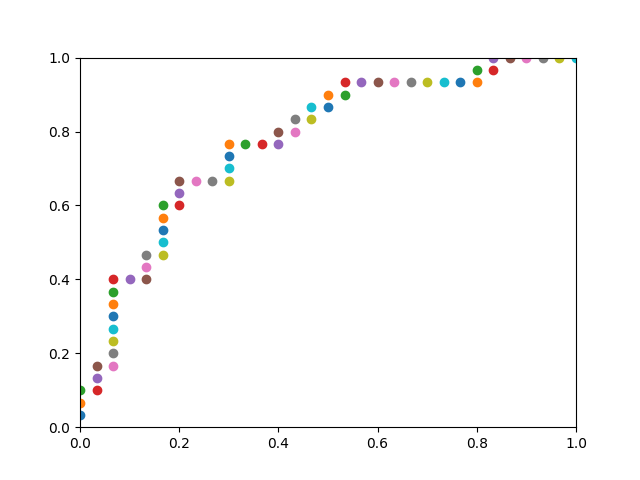
\includegraphics[scale=0.3]{ROC.png}
\caption{ROC krivulja}
\label{slika4}
\end{center}
\end{figure}

\section{Izbor značilk.}
/

\end{document}
